\section{Test session}
\label{TestSessionValgAfGestikker}
%
Testens varighed afhænger af testpersonernes respons, men anslåes til at vare mellem et kvarter og en halv time, inklusiv testlederens instruktioner og det afsluttende exit-interview.

Test sessionen begynder med at testlederen byder testpersonen velkommen og introducerer testpersonen til hvad der kommer til at foregå undervejs i testen og at det ønskes at optage testpersonen undervejs, hvorefter testpersonen får udleveret en samtykkeerklæring, som de opfordres til at læse og underskrive. Så snart samtykkeerklæringen er underskrevet starter testlederen videokameraet. Dernæst bliver testpersonerne bedt om at udfylde spørgeskemaet, hvor de opfordres til at stille spørgsmål hvis der opstår tvivl. Inden testen påbegyndes bliver testpersonerne yderligere instrueret i hvad der kommer til at foregå samt hvilke opgaver de skal løse. Når testpersonerne har gennemgået de tre videoer og løst de pågældende opgaver, afvikles exit-interviewet. 
%

\section{Testpersoner}
\label{TestpersonerValgAfGestikker}
%
Testen udføres på studerende fra Aalborg Universitet. Det tilstræbes ikke at teste på studerende med forhåndsviden om design, brugertest og lignende eller studerende, hvis hovedfokus er elektronik og software, da det antages at denne målgruppe primært vil fokusere på teknologien bag produktet eller andre specifikke designaspekter og derfor ikke vil være i stand til at give upåvirket respons, \parencite[s. 110]{Book:OUE}. 

Ifølge Bang $\&$ Olufsen vil studerende fra Aalborg Universitet være en repræsentativ målgruppe, hvorfor der ikke sættes yderligere krav til testpersonerne, jævnfør \autoref{app:InterviewLyleClarke}.  
%

\section{Rollefordeling}
\label{RollerfordelingValgAfGestikker}
%
For at udføre testen skal der udpeges to roller; en testleder og en observatør. Testlederens opgave er at instruere testpersonerne om hvordan testen vil forløbe, opfordre testpersonerne til at læse og underskrive samtykkeerklæringen, starte optagelsen efter testpersonerne har underskrevet samtykkeerklæringen, sørger for at testpersonerne udfylder spørgeskemaet, formidle testpersonernes opgaver samt at afvikle exit-interviewet. Testlederens instruktioner fremgår af \autoref{app:InstruktionerValgAfGestikker} og samtykkeerklæringen fremgår af BILAG. 

Observatørens opgave er at tage noter til testpersonernes respons og sørger for at pause og starte musikken, skift musiknummer frem og tilbage samt skrue op og ned for musikken når testpersonerne opfordres til at forbedre deres fortrukne gestik til den specifikke video og når de afslutningsvist opfordres til at gengive gestikkerne igen. 

\section{Udstyr og testlokation}
\label{UdstyrOgTestlokationValgAfGestikker}
%
Til testen indgår følgende udstyr:
%
\begin{itemize}
  \item Videokamera + stativ
  \item Tre videoer med gestikker
  \item Ekstern farveskærm 
  \item To højtalere
  \item iTunes 12.6  
  \item Computer med internetforbindelse\blankline
\end{itemize}
% 
Videokamera og stativ indgår da det ønskes at optage testpersonernes forbedringerne til at pause og starte musikken, skrue op og ned for musikken og til at skift musiknummer frem og tilbage. Ydermere benyttes videokameraet til at optage testpersonernes respons undervejs og afslutningsvist i exit-interviewet. Det er derfor essentielt at videokameraet kan optage lyd og at videokameraet placeres dels så det kan optage testpersonernes bevægelser og dels optage deres orale respons. De tre videoer med gestikker er optaget på forhånd og gengiver, parvist, de seks mest gængse funktioner på et musikanlæg. Farveskærmen indgår for at præsenterer de tre videoer på en skærm, der er større end skærmen på en bærbar computer. De to højtalere skal tilkobles computeren hvorfra skærmen, hvor videoerne afspilles på, ligeledes er koblet til. De to højtalere er af typen Genelec 1031A, da er fast inventar i lokalet hvor testen afvikles. iTunes 12.6 indgår i forbindelse med at testpersonerne opfordres til at forbedre deres fortrukne gestik og afslutningsvist hvor de opfordres til at gengive gestikkerne igen. Computer med internetforbindelse er nødvendig da det er der testpersonerne skal udfylde spørgeskemaet, i denne opstilling er det også den computer hvor den eksterne farveskærm og de to højtalere er tilkoblet. \autoref{fig:TestopstillingPrePilot} gengiver testopstillingen.  
%
\begin{figure}[H]
	\centering
	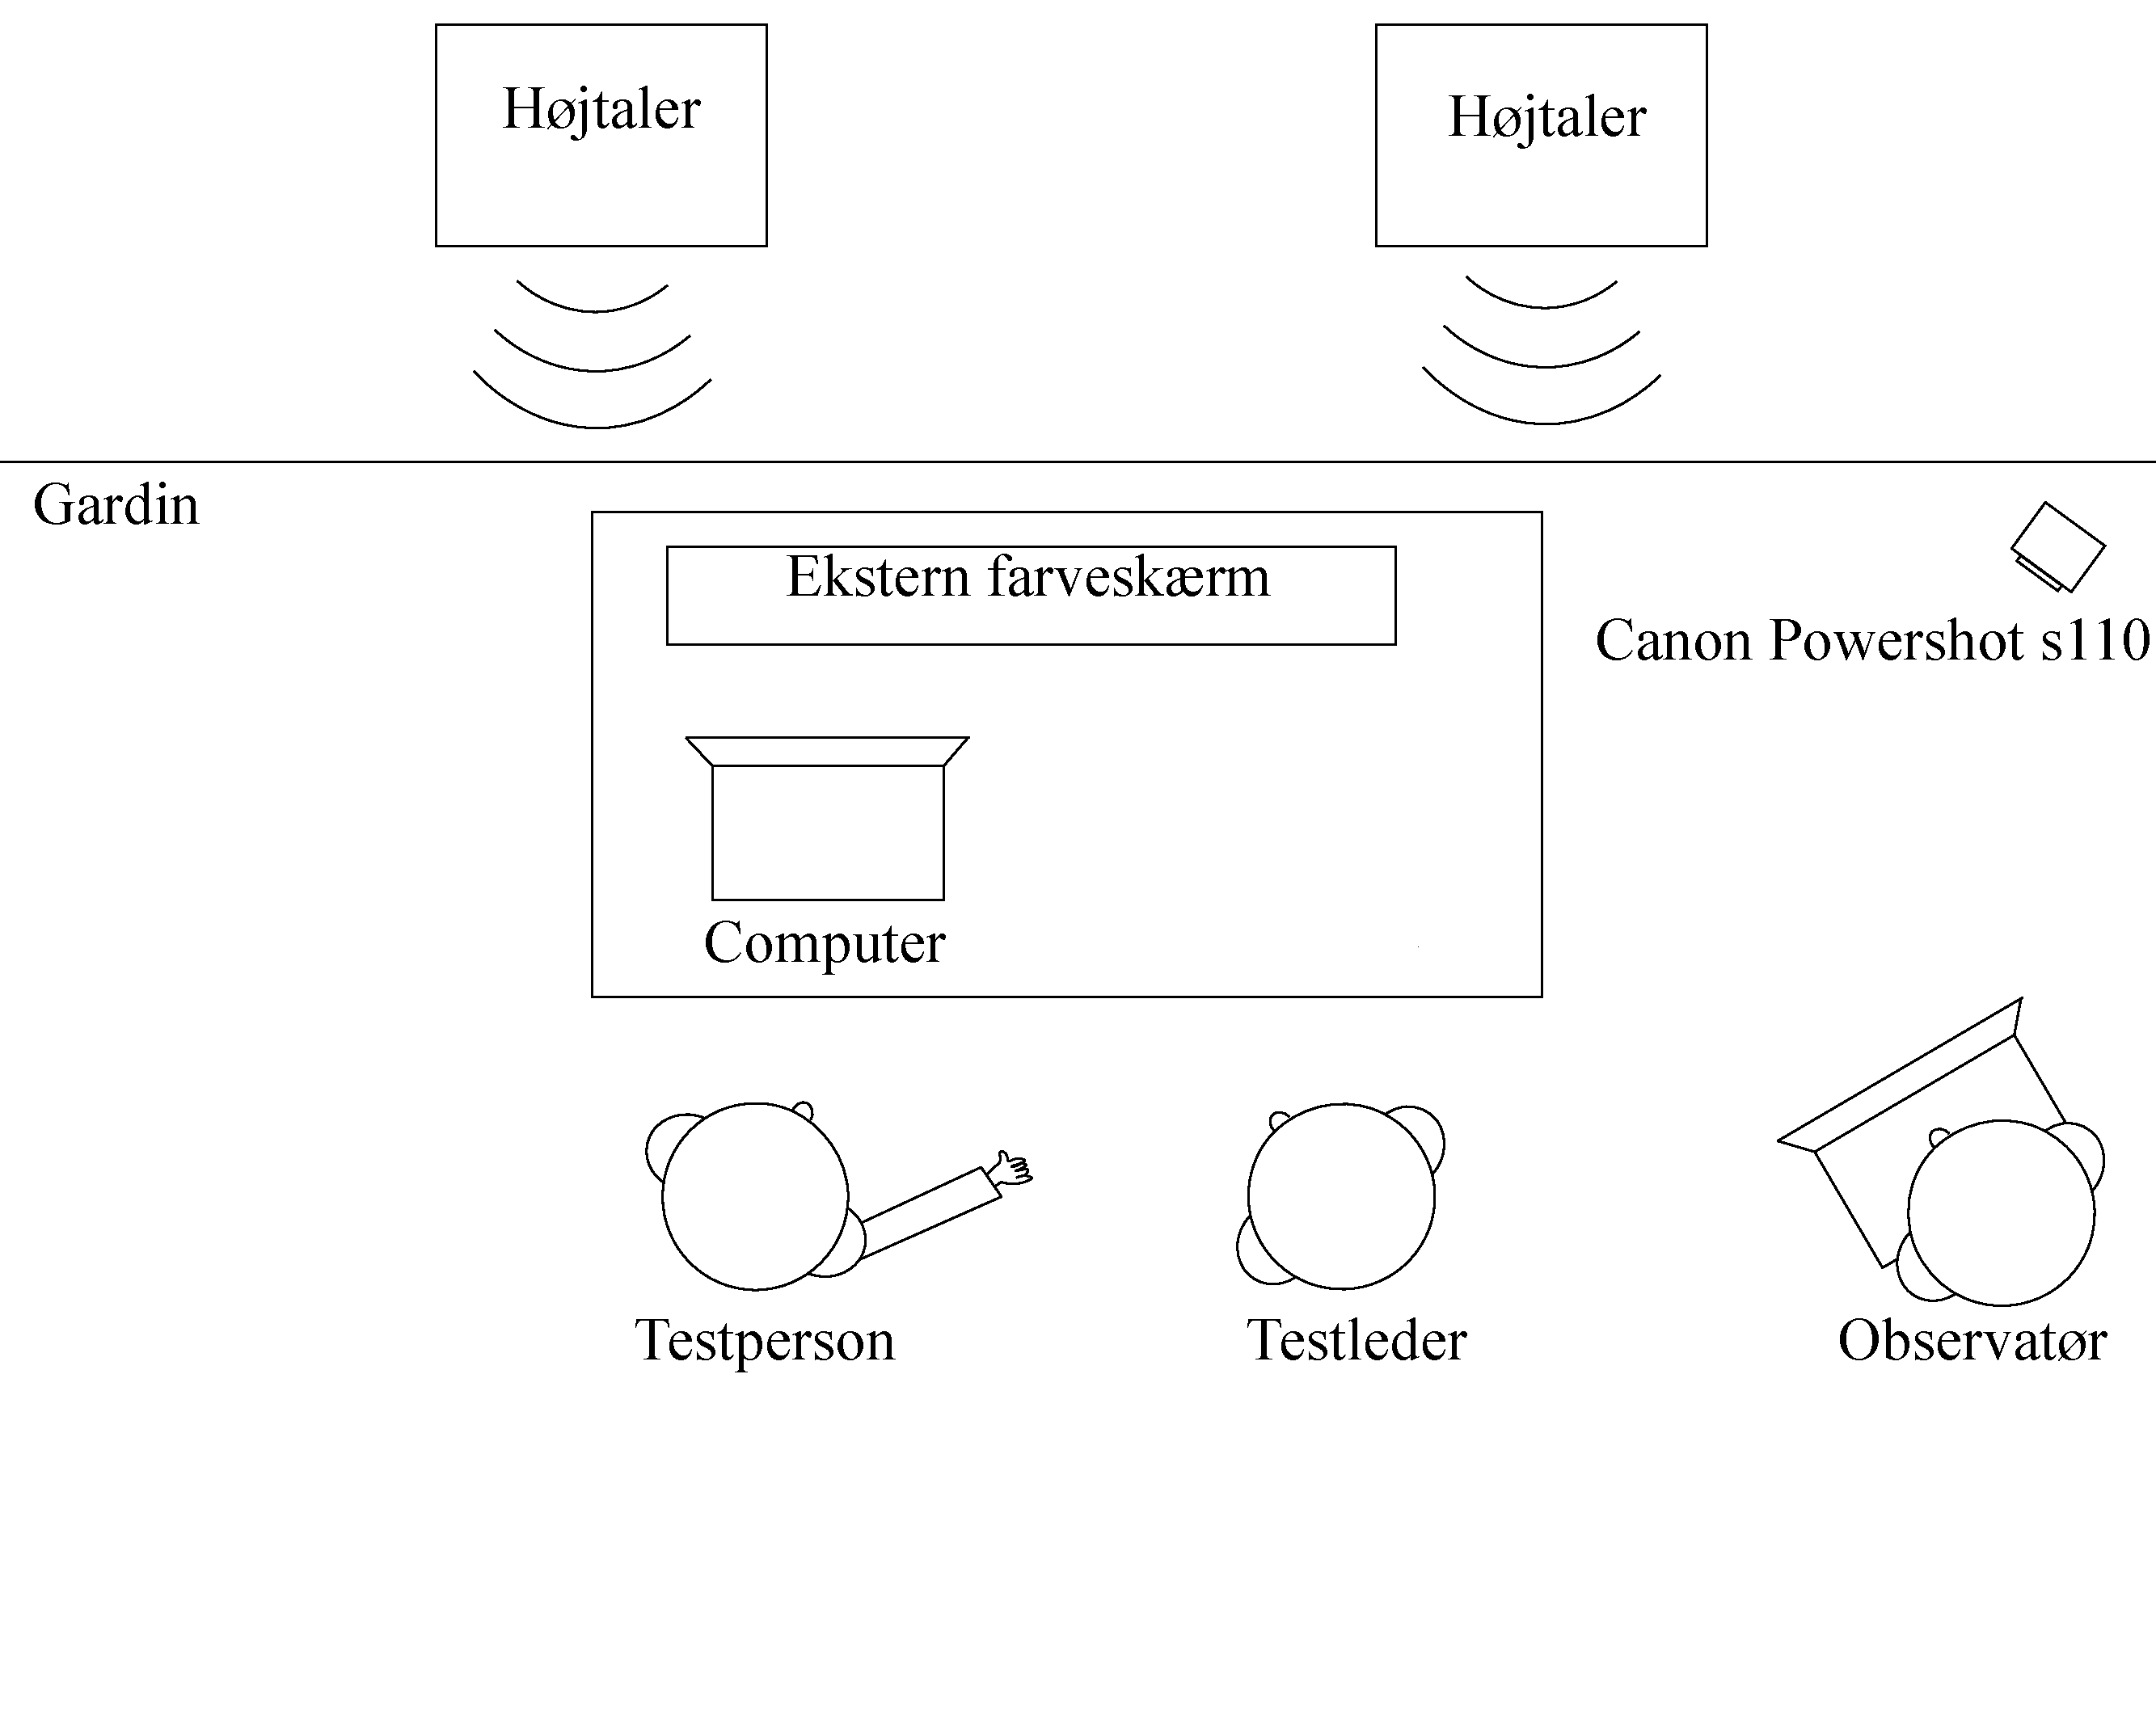
\includegraphics[resolution=300,width=0.8\textwidth]{Test1/TestopstillingPrePilot}
	\caption{Testopstilling hvor placeringen af udstyr, testleder, observatør og testperson fremgår.}
	\label{fig:TestopstillingPrePilot}
\end{figure}
\noindent
% 
Testen afvikles i akustikafdelingen på Aalborg Universitet, Fredrik Bajers Vej 7B, i lokale: Lytterummet B4-107. 
%